\chapter{Apêndice}\label{chapter:apendice}

% -----------------------------------------------------------------------------
% Capítulo X.1 - Kits de Desenvolvimento
% -----------------------------------------------------------------------------
\section{Kits de Desenvolvimento}\label{section:kits_de_desenvolvimento}

As tabelas \autoref{table:development_kit_a} e \autoref{table:development_kit_b} mostram os parâmetros de cinco kits de desenvolvimento cogitados para serem o protótipo do projeto.

\begin{table}[H]
    \begin{tblr}{@{}|X[c,valign=m,gray!30]|X[c,valign=m]|X[c,valign=m]|X[c,valign=m]|X[c,valign=m]|X[c,valign=m]|@{}}
        \hline
        \textbf{Número de produto}        & B-L475E-IOT01A2                                                           & CORE-V MCU DevKit                                                   & SLN-ALEXA-IOT                                  \\ \hline
        \textbf{Descrição}                & STM32L4 Discovery kit Nó IoT, low-power wireless, BLE, NFC, SubGHz, Wi-Fi & European RISC-V chip for IoT development kit                        & EdgeReady MCU Based Solution for Alexa for IOT \\ \hline
        \textbf{Processador}              & Arm® Cortex®-M4                                                           & CV32E40P processor core                                             & Arm® Cortex®-M7 Core                           \\ \hline
        \textbf{FreeRTOS}                 & Sim                                                                       & Não Disponível                                                      & Sim                                            \\ \hline
        \textbf{Conectividade}            & Inventek ISM43362 Wi-Fi Module                                            & Espressif AWS IoT ExpressLink Module for AWS IoT cloud interconnect & Bluetooth LE 4.2, 802.11 b/g/n Wi-Fi®          \\ \hline
        \textbf{Microfones}               & 2 digital omnidirectional microphones (MP34DT01)                          & Não Disponível                                                      & Digital MEMS microphones (x3)                  \\ \hline
        \textbf{Alto-falante}             & Não Disponível                                                            & Não Disponível                                                      & Não Disponível                                 \\ \hline
        \textbf{Preço nas Lojas Oficiais} & \$53,00                                                                   & Preços Individuais                                                  & \$171,35                                       \\ \hline
    \end{tblr}
    \caption{kits de desenvolvimento recomendados pela Amazon para o desenvolvimento de aplicações IoT (A).}
    \label{table:development_kit_a}
\end{table}

\begin{table}[H]
    \begin{tblr}{@{}|X[c,valign=m,gray!30]|X[c,valign=m]|X[c,valign=m]|X[c,valign=m]|X[c,valign=m]|X[c,valign=m]|@{}}
        \hline
        \textbf{Número de produto}        & Home Hub 100 Dev Kit for Amazon AVS                                                                                                                                             & STEVAL-VOICE-UI                                                                                                                                                            \\ \hline
        \textbf{Descrição}                & A hardware and software development kit with multi-core connectivity designed to support AVS for AWS IoT Core connected devices                                                 & Qualified hardware reference design enabling easy and cost effective addition of the Alexa Voice Service (AVS) Integration for AWS IoT core to your smart embedded devices \\ \hline
        \textbf{Processador}              & Arm Cortex-M4F CPU                                                                                                                                                              & Dual Arm® Cortex®-A7 and Cortex®-M4 Cores                                                                                                                                  \\ \hline
        \textbf{FreeRTOS}                 & Sim                                                                                                                                                                             & Sim                                                                                                                                                                        \\ \hline
        \textbf{Conectividade}            & Integrated Bluetooth 5, Qualcomm® Bluetooth Mesh connectivity, low power Wi-Fi 802.11n in 2.4GHz/5GHz bands, and 802.15.4, with support for ZigBee3.0 and Thread via OpenThread & WIFI subsystem including Murata 1DX module used in bypass mode and ISSI IS25LP016D 2Mbytes NOR flash hosting WIFI low level software                                       \\ \hline
        \textbf{Microfones}               & Não Disponível                                                                                                                                                                  & 2 MP23DB01HP Microphone Mems                                                                                                                                               \\ \hline
        \textbf{Alto-falante}             & 1x                                                                                                                                                                              & 1x (8 ohm)                                                                                                                                                                 \\ \hline
        \textbf{Preço nas Lojas Oficiais} & £42.95                                                                                                                                                                          & \$248.75                                                                                                                                                                   \\ \hline
    \end{tblr}
    \caption{kits de desenvolvimento recomendados pela Amazon para o desenvolvimento de aplicações IoT (B).}
    \label{table:development_kit_b}
\end{table}

% -----------------------------------------------------------------------------
% Capítulo X.2 - Criação de uma política IAM
% -----------------------------------------------------------------------------
\section{Criação de uma política para o AWS IoT}\label{section:criacao_de_uma_politica_para_o_aws_iot}

A sequência de figuras apresentam capturas de telas do processo de criação de uma política para o AWS IoT.

Acesse a \href{https://us-east-1.console.aws.amazon.com/iot/home?region=us-east-1#/home}{página principal do serviço AWS IoT}, expanda a opção \textit{Segurança} e selecione \textit{Políticas}.

\begin{figure}[H]
    \centering
    \caption{Criando uma política no AWS IoT (A).}
    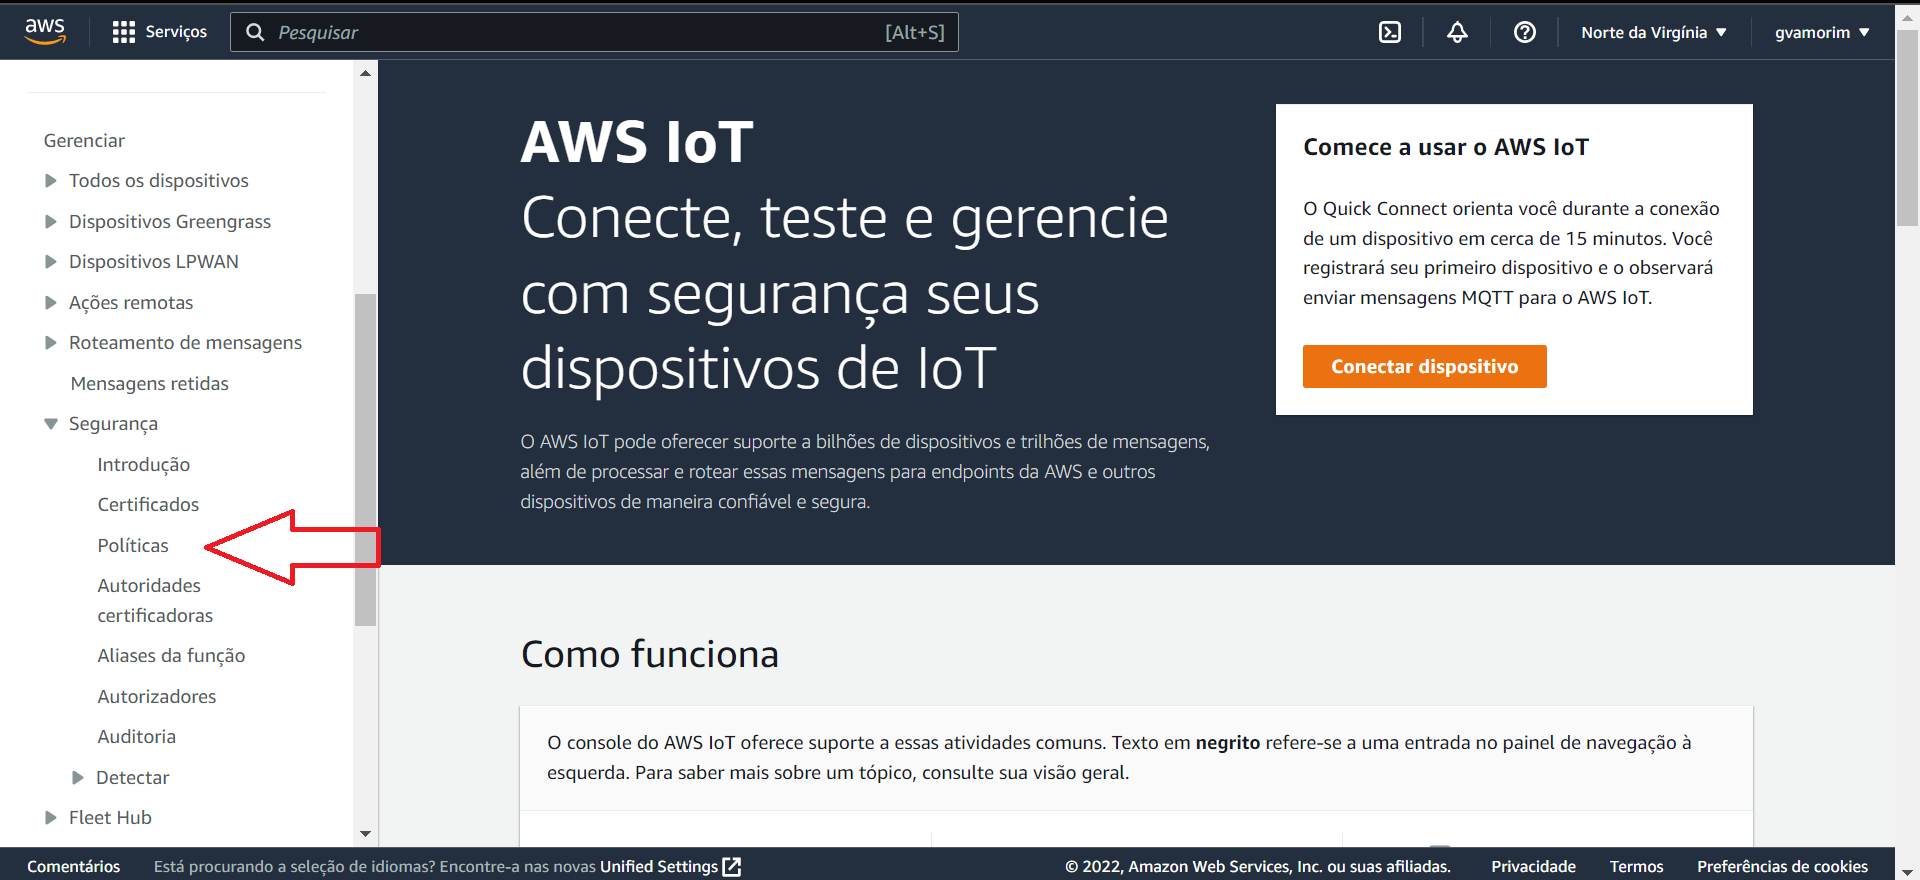
\includegraphics[scale=0.472]{Imagens/criando_uma_politica_no_aws_iot_0.png}
    \legend{Fonte: Produzido pelo autor (2022).}
    \label{fig:criando_uma_politica_no_aws_iot_a}
\end{figure}

Selecione a opção \textit{Criar política}.

\begin{figure}[H]
    \centering
    \caption{Criando uma política no AWS IoT (B).}
    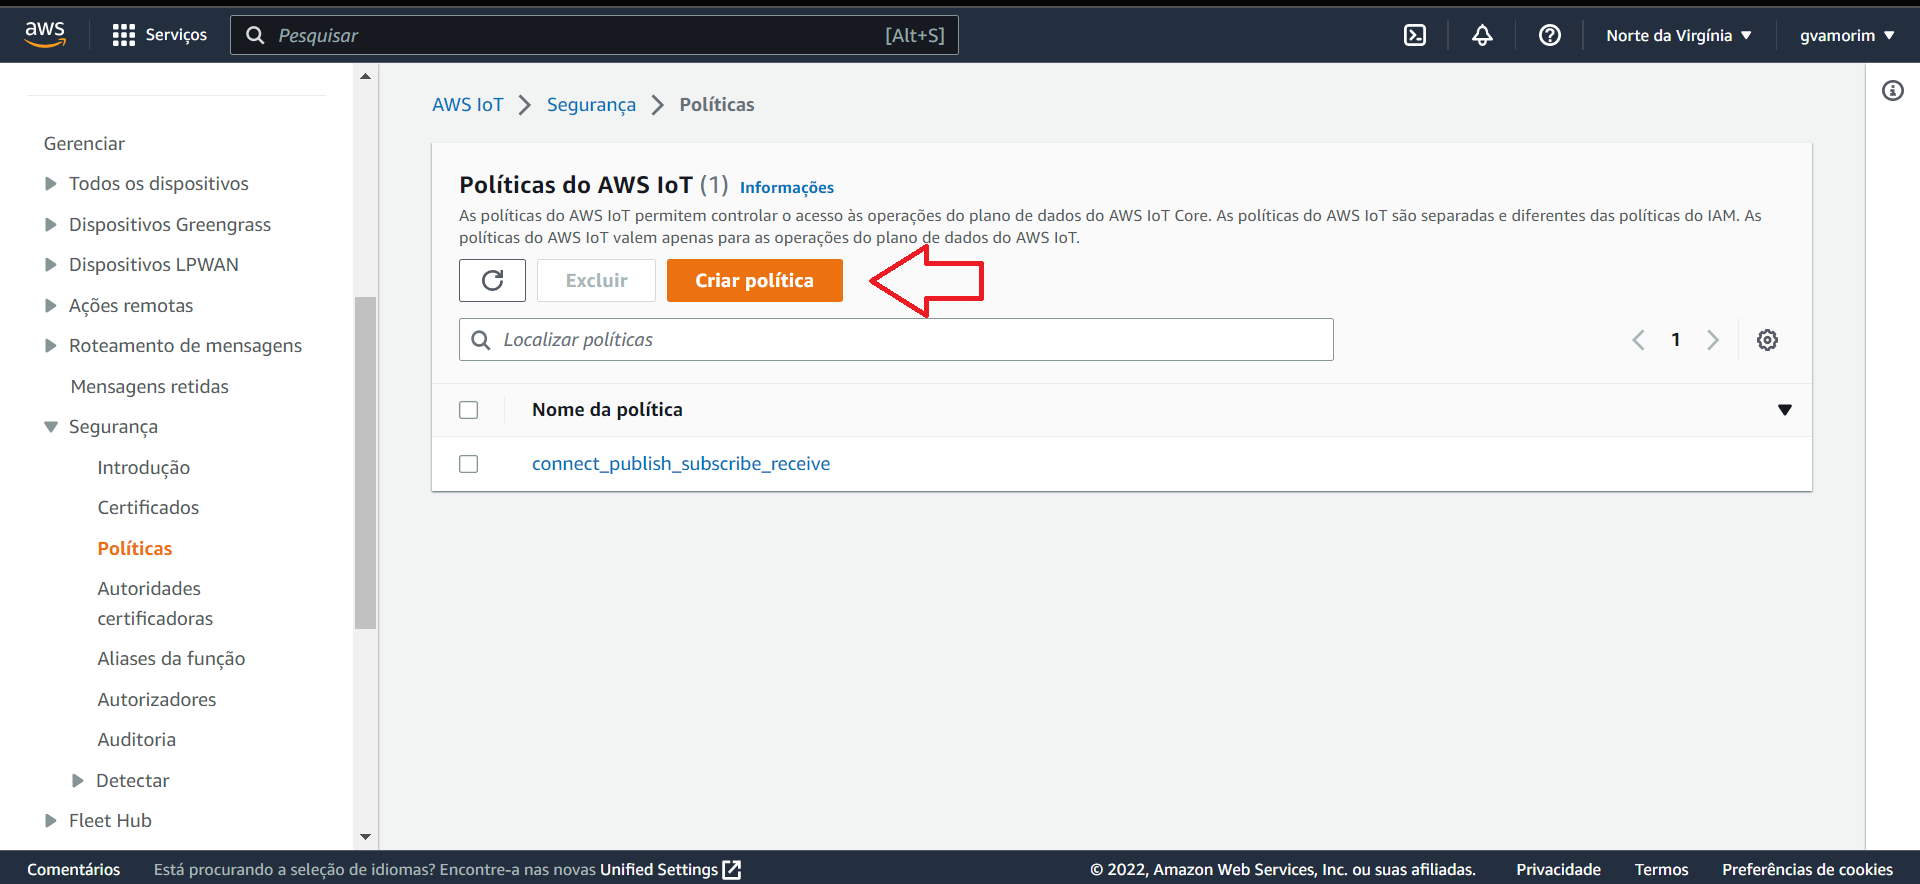
\includegraphics[scale=0.472]{Imagens/criando_uma_politica_no_aws_iot_1.png}
    \legend{Fonte: Produzido pelo autor (2022).}
    \label{fig:criando_uma_politica_no_aws_iot_b}
\end{figure}

Adicione um nome na opção \textit{Nome da política}.

\begin{figure}[H]
    \centering
    \caption{Criando uma política no AWS IoT (C).}
    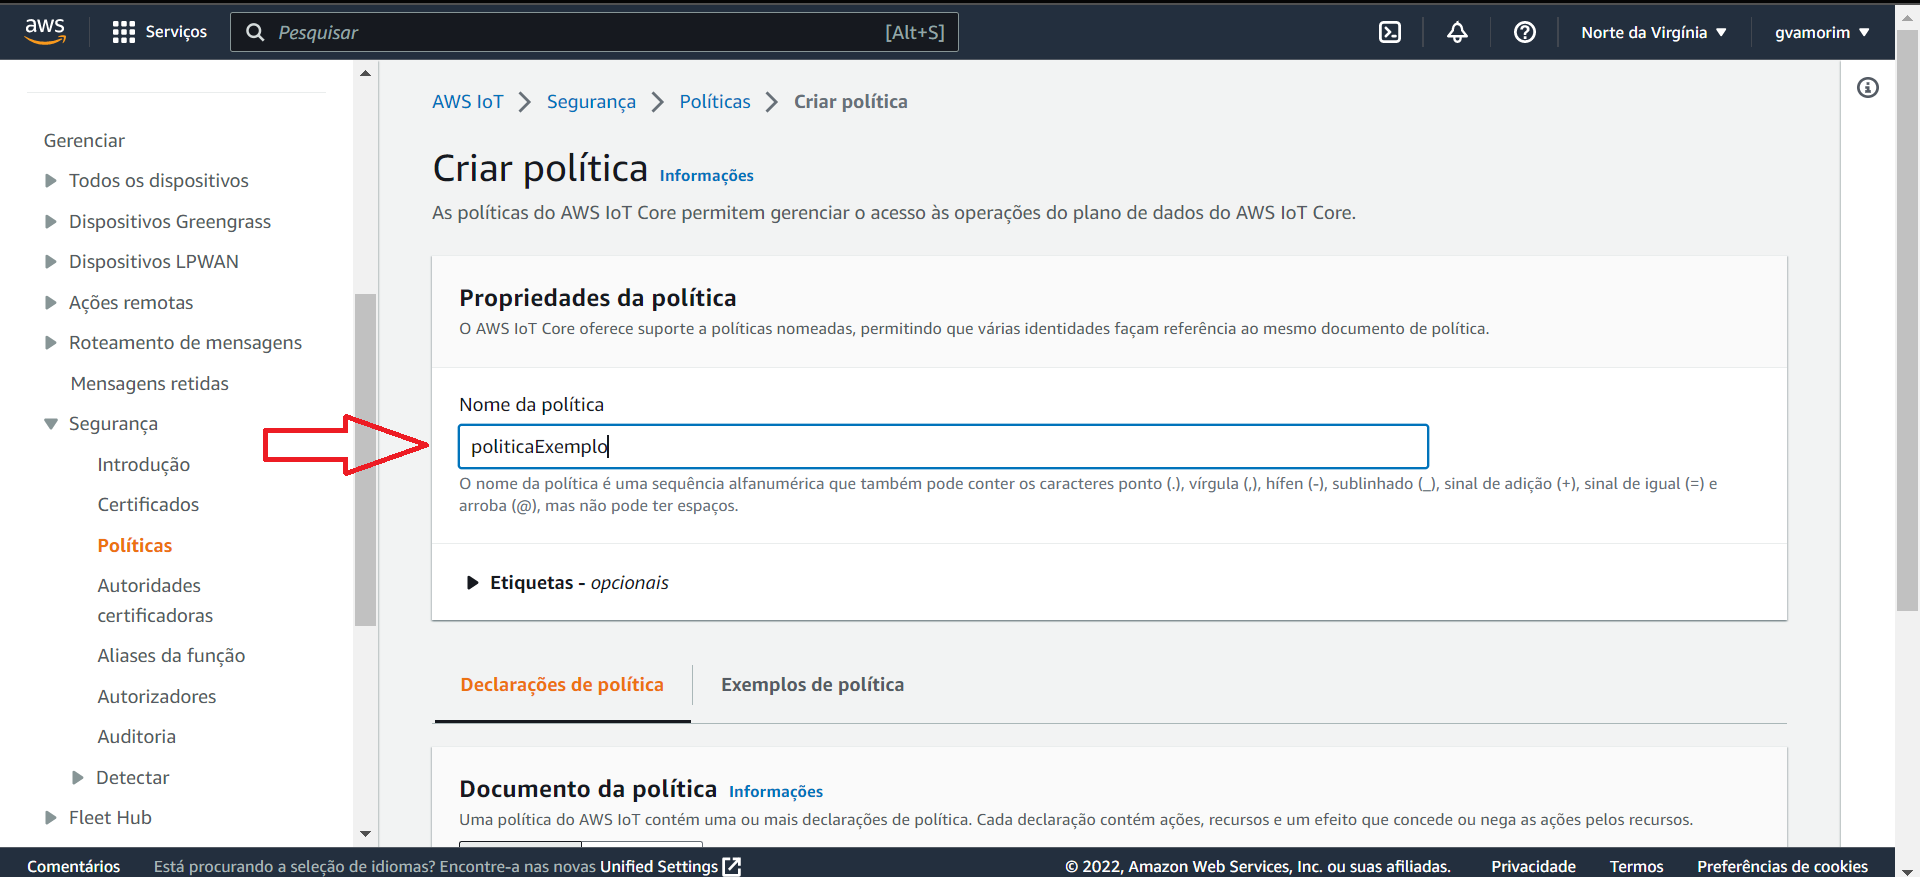
\includegraphics[scale=0.472]{Imagens/criando_uma_politica_no_aws_iot_2.png}
    \legend{Fonte: Produzido pelo autor (2022).}
    \label{fig:criando_uma_politica_no_aws_iot_c}
\end{figure}

Adicione declarações à política. As declarações podem ser adicionadas iterativamente (\autoref{fig:criando_uma_politica_no_aws_iot_d}) ou via documento JSON (\autoref{fig:criando_uma_politica_no_aws_iot_e}). O documento JSON da política utilizada no projeto foi apresentado no \autoref{lst:bl475e_policy}. Note que a opção \textit{Resource}, para cada declaração, segue o seguinte formato: ``arn:aws:iot: \textless regiao\textgreater:\textless id\_do\_usuario\textgreater:*''.

\begin{figure}[H]
    \centering
    \caption{Criando uma política no AWS IoT (D).}
    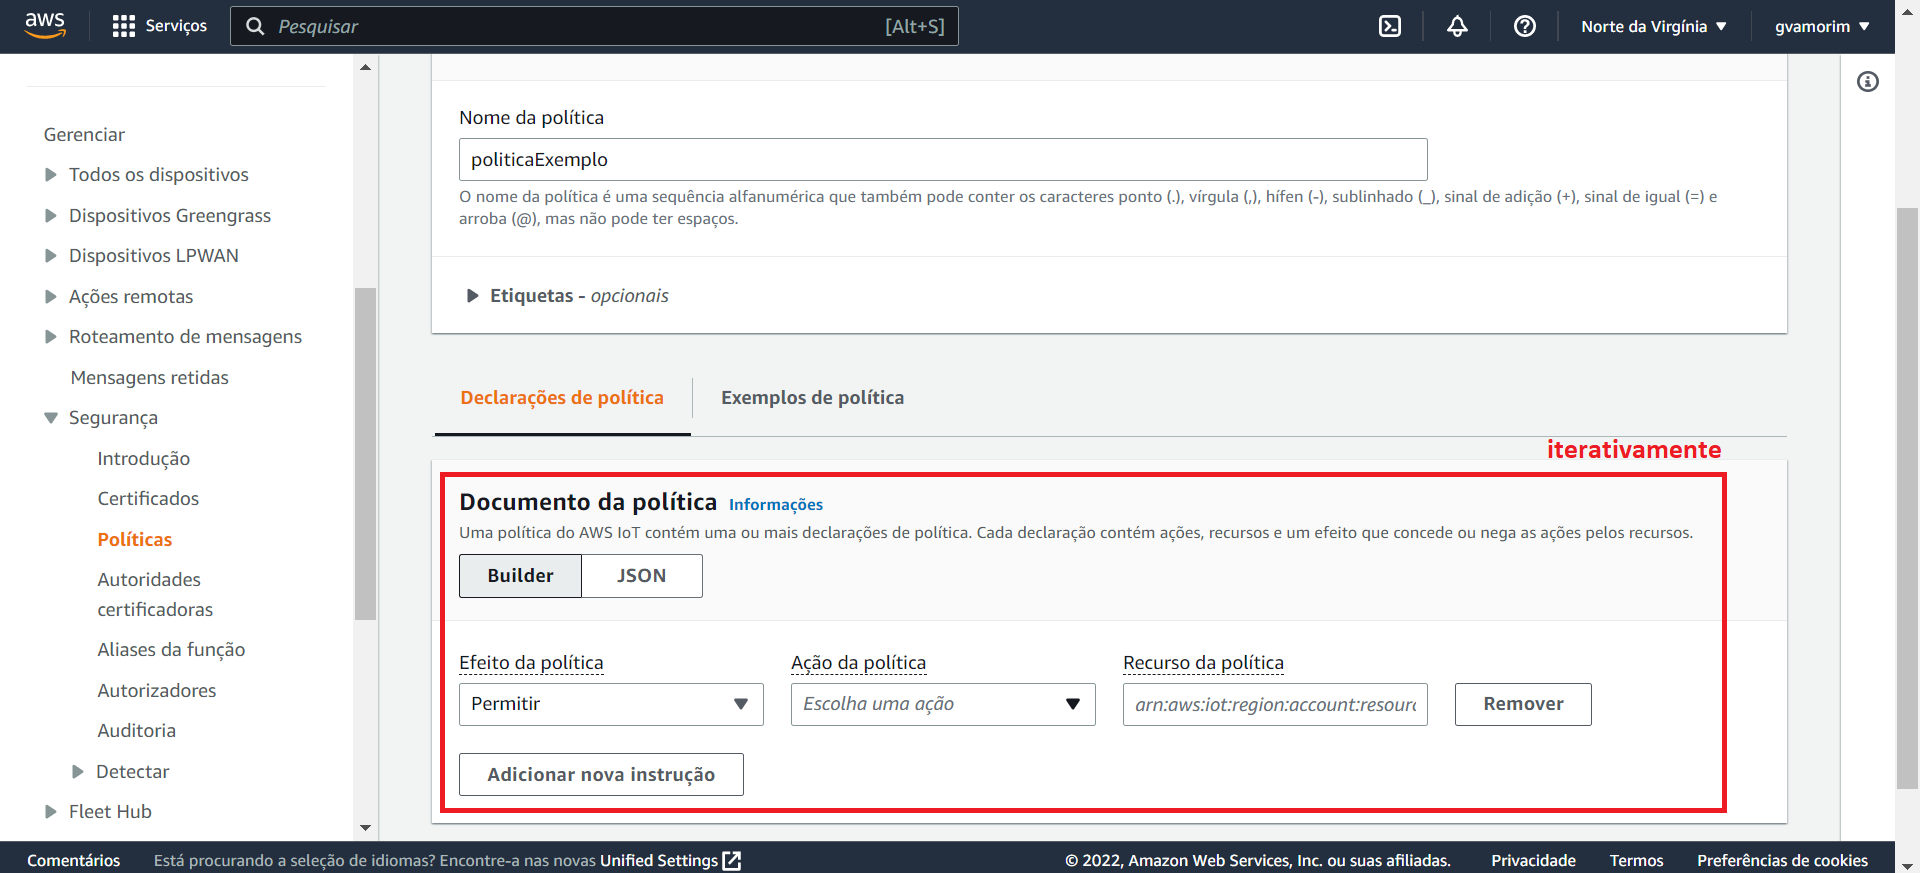
\includegraphics[scale=0.472]{Imagens/criando_uma_politica_no_aws_iot_3.png}
    \legend{Fonte: Produzido pelo autor (2022).}
    \label{fig:criando_uma_politica_no_aws_iot_d}
\end{figure}

\begin{figure}[H]
    \centering
    \caption{Criando uma política no AWS IoT (E).}
    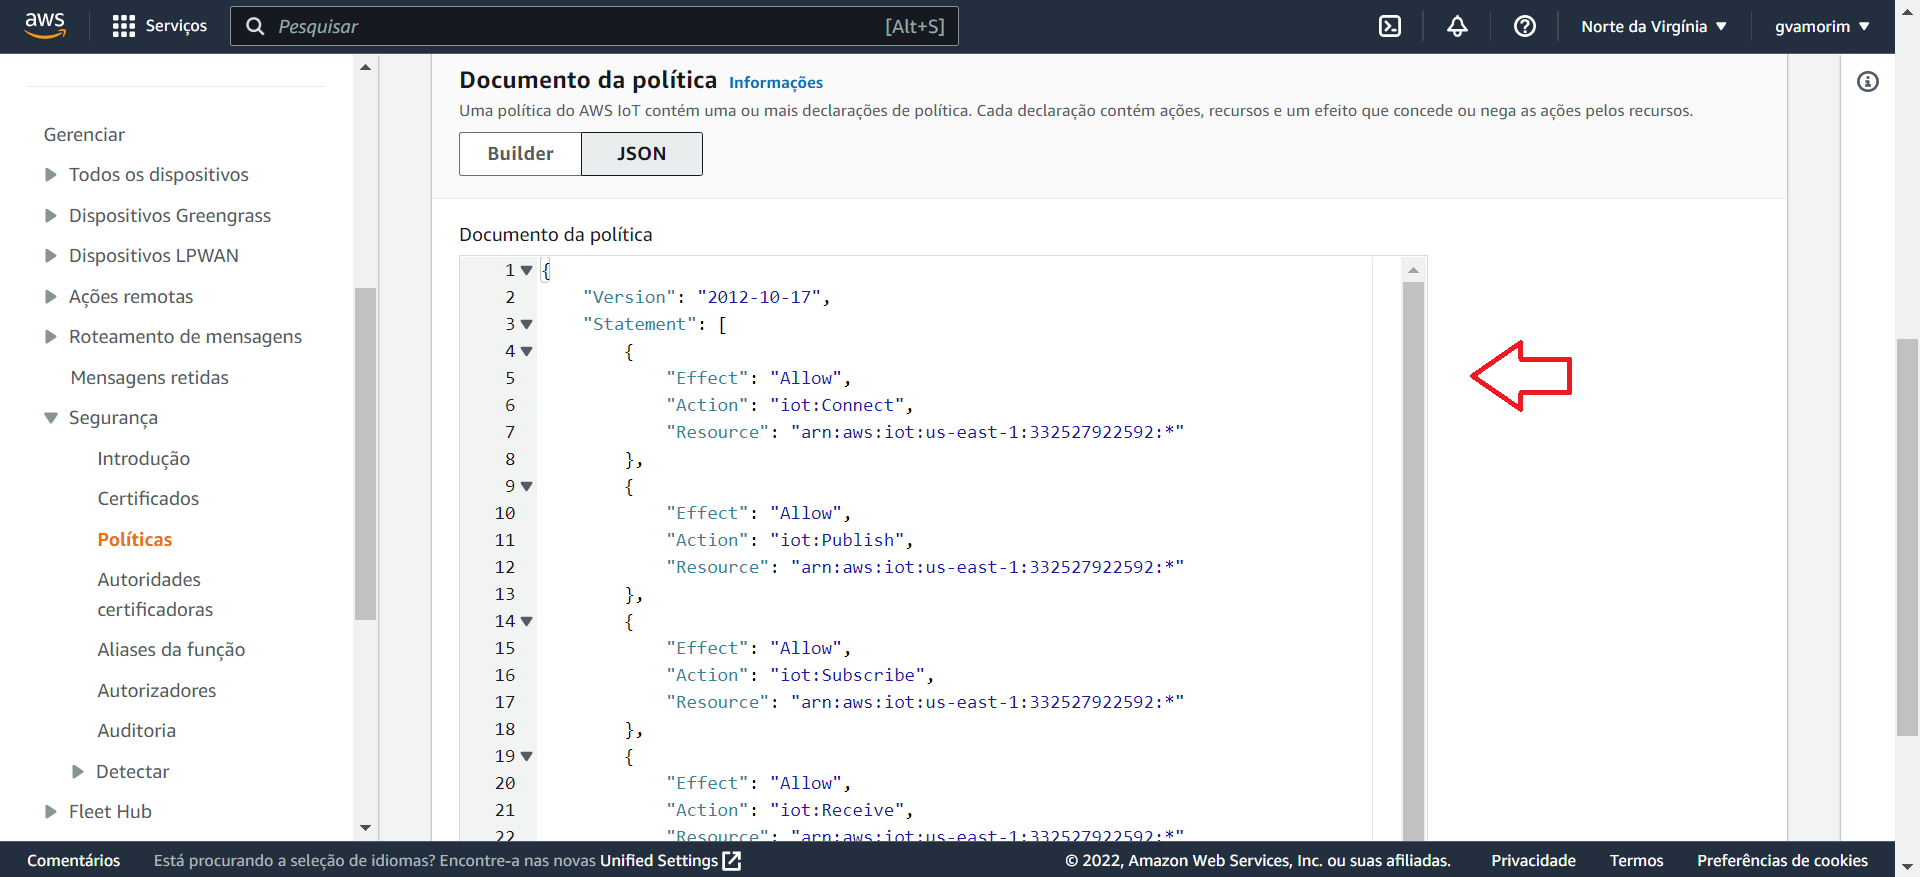
\includegraphics[scale=0.472]{Imagens/criando_uma_politica_no_aws_iot_4.png}
    \legend{Fonte: Produzido pelo autor (2022).}
    \label{fig:criando_uma_politica_no_aws_iot_e}
\end{figure}

Selecione a opção \textit{Criar}.

\begin{figure}[H]
    \centering
    \caption{Criando uma política no AWS IoT (F).}
    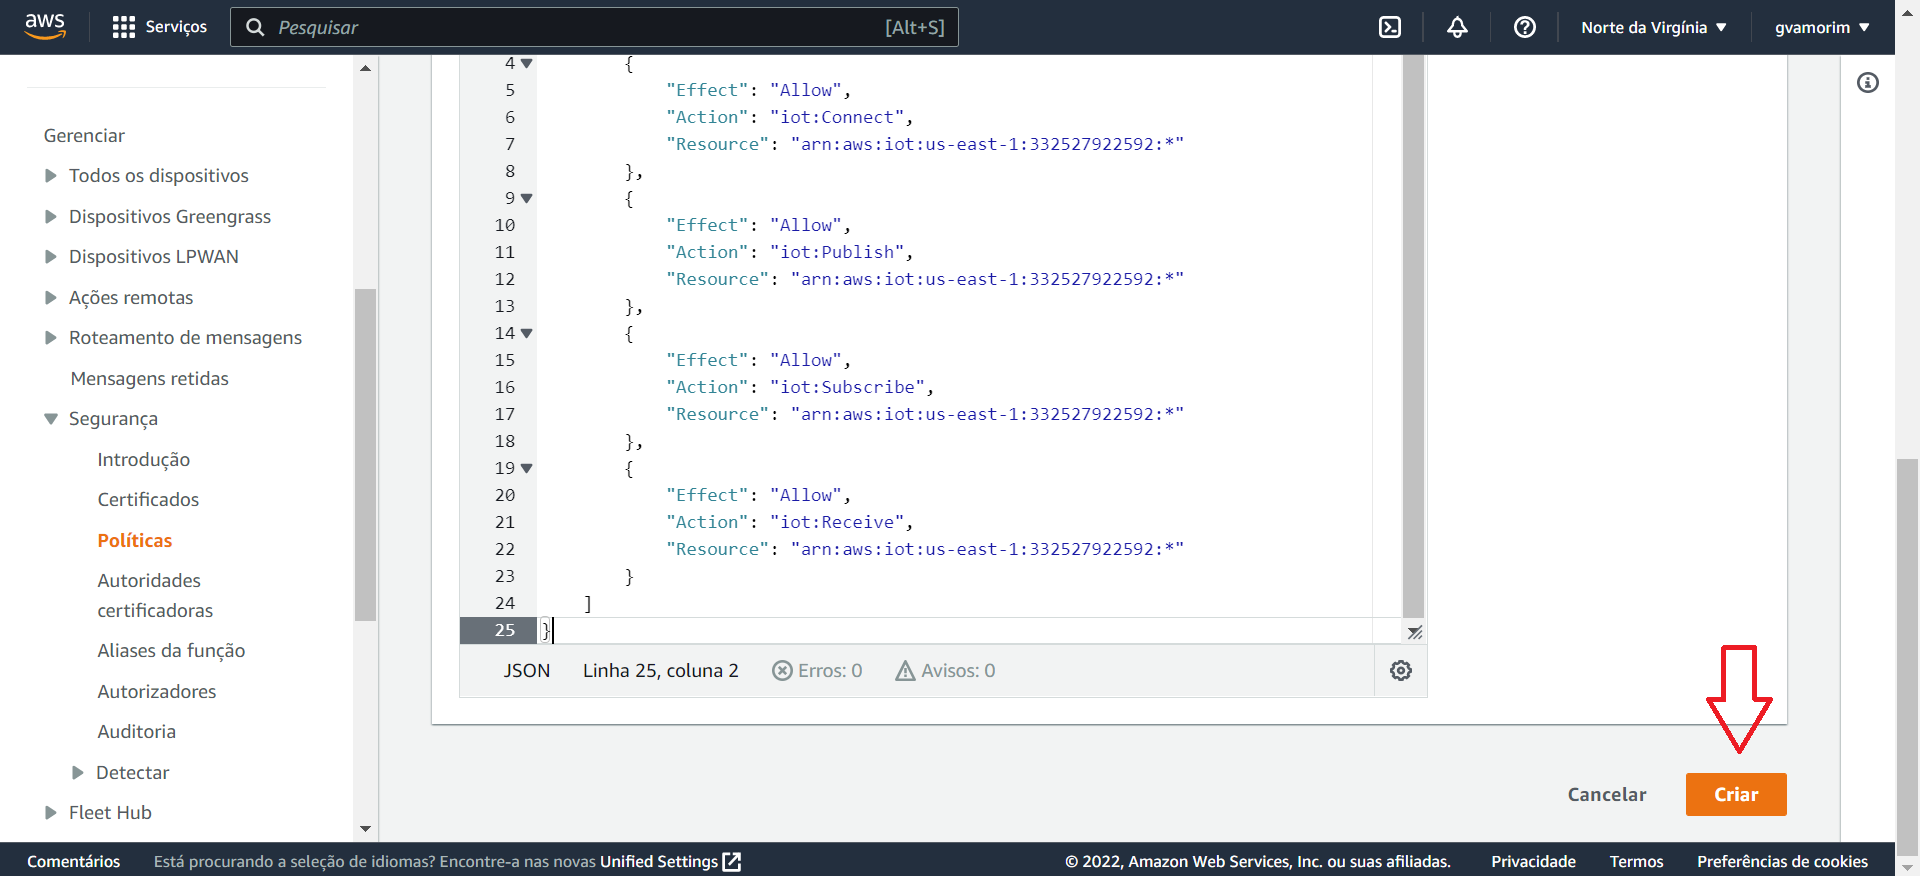
\includegraphics[scale=0.472]{Imagens/criando_uma_politica_no_aws_iot_5.png}
    \legend{Fonte: Produzido pelo autor (2022).}
    \label{fig:criando_uma_politica_no_aws_iot_f}
\end{figure}


% -----------------------------------------------------------------------------
% Capítulo X.2 - Criação de uma coisa no AWS IoT
% -----------------------------------------------------------------------------
\section{Criação de uma coisa no AWS IoT}\label{section:criacao_de_uma_coisa_no_aws_iot}

A sequência de figuras \autoref{fig:criacao_de_uma_coisa_no_aws_iot_a} até \autoref{fig:criacao_de_uma_coisa_no_aws_iot_g} apresentam capturas de telas do processo de criação de uma coisa no AWS IoT.

Acesse a \href{https://us-east-1.console.aws.amazon.com/iot/home?region=us-east-1#/home}{página principal do serviço AWS IoT}, expanda a opção \textit{Todos os Dispositivos} e selecione \textit{coisas}.

\begin{figure}[H]
    \centering
    \caption{Criando uma coisa no AWS IoT (A).}
    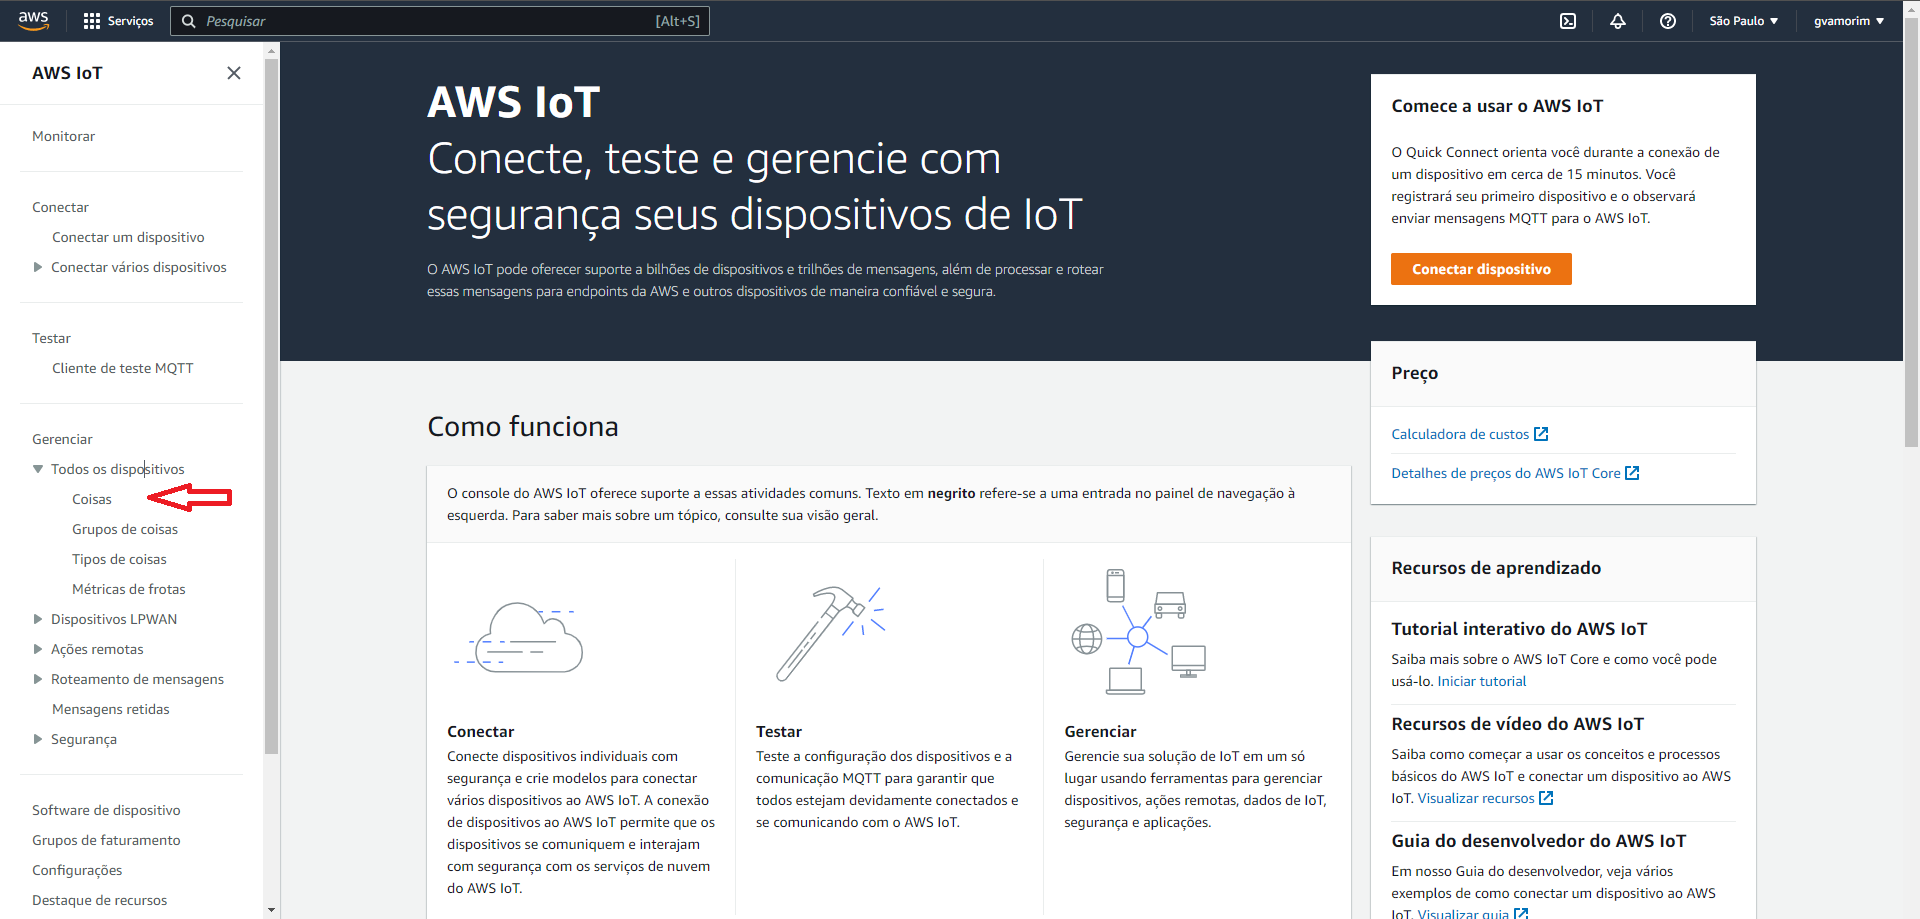
\includegraphics[scale=0.315]{Imagens/criando_uma_coisa_no_aws_iot_0.png}
    \legend{Fonte: Produzido pelo autor (2022).}
    \label{fig:criacao_de_uma_coisa_no_aws_iot_a}
\end{figure}

Selecione a opção \textit{Criar items}.

\begin{figure}[H]
    \centering
    \caption{Criando uma coisa no AWS IoT (B).}
    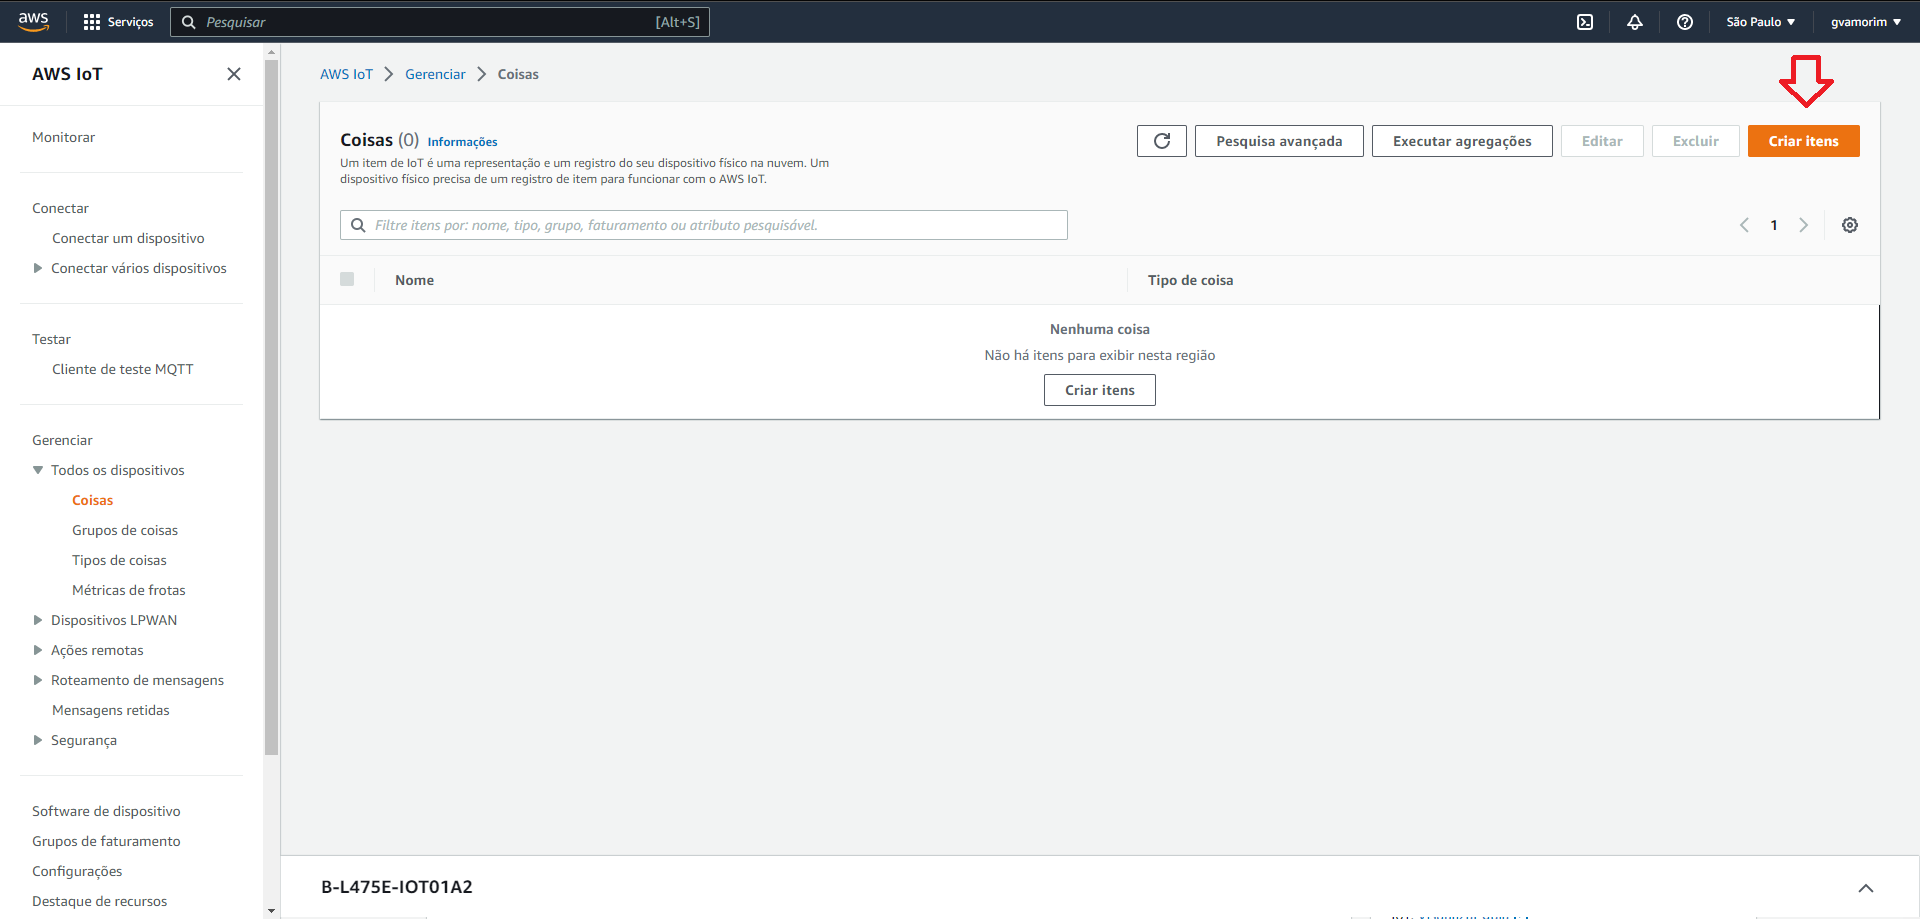
\includegraphics[scale=0.315]{Imagens/criando_uma_coisa_no_aws_iot_1.png}
    \legend{Fonte: Produzido pelo autor (2022).}
\end{figure}

Selecione a opção \textit{Criar um único item}.

\begin{figure}[H]
    \centering
    \caption{Criando uma coisa no AWS IoT (C).}
    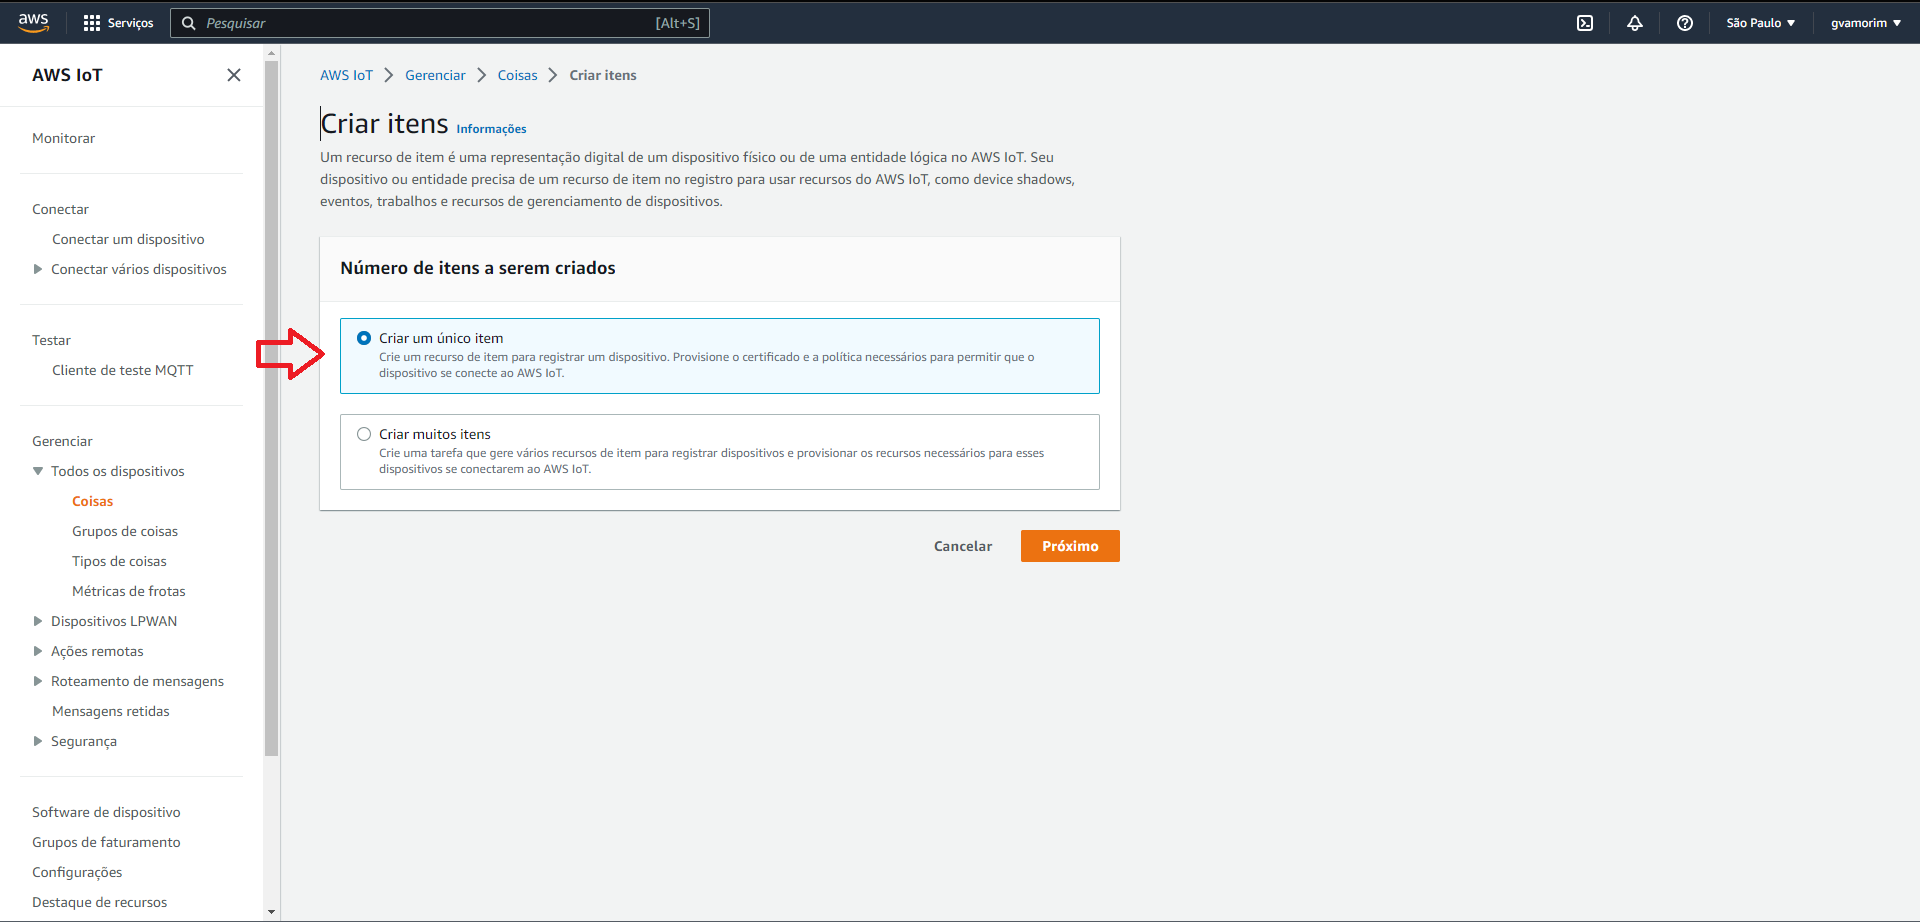
\includegraphics[scale=0.315]{Imagens/criando_uma_coisa_no_aws_iot_2.png}
    \legend{Fonte: Produzido pelo autor (2022).}
\end{figure}

Adicione um nome na opção \textit{Nome da coisa} e selecione \textit{Sombra sem nome (clássico)}.

\begin{figure}[H]
    \centering
    \caption{Criando uma coisa no AWS IoT (D).}
    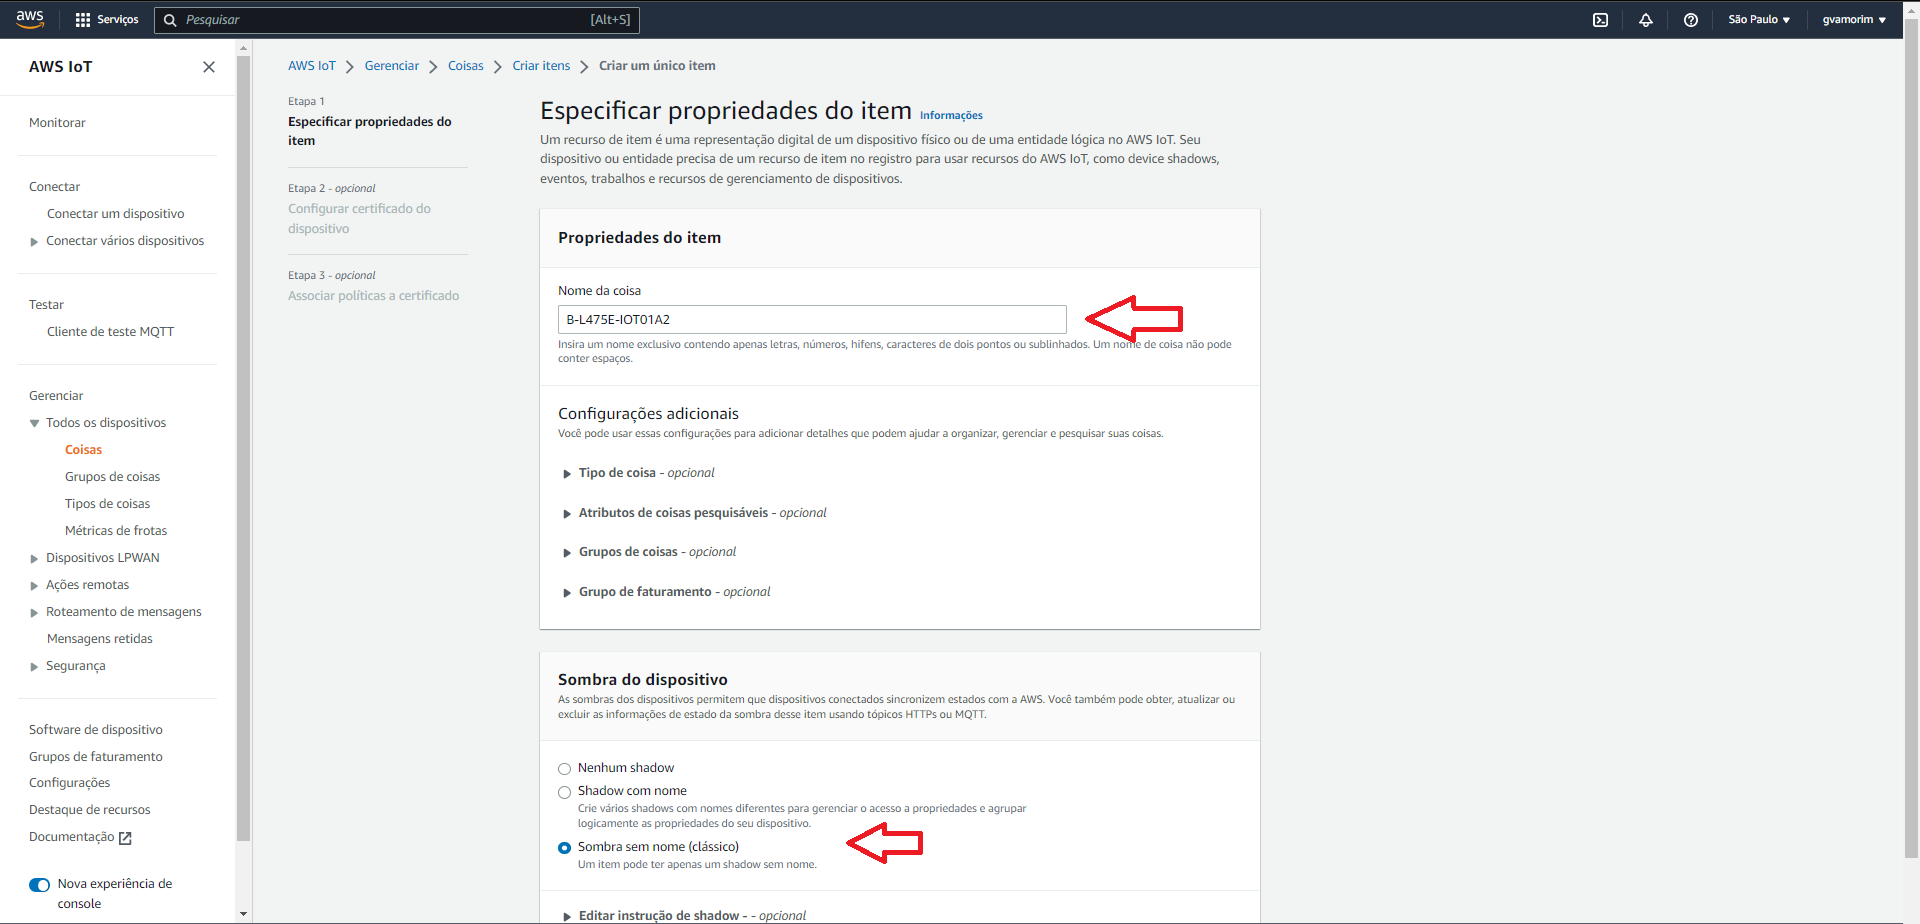
\includegraphics[scale=0.315]{Imagens/criando_uma_coisa_no_aws_iot_3.png}
    \legend{Fonte: Produzido pelo autor (2022).}
\end{figure}

Selecione a opção \textit{Gerar um novo certificado automaticamente (recomendado)}. Um dispositivo requer um certificado para conectar-se ao AWS IoT.

\begin{figure}[H]
    \centering
    \caption{Criando uma coisa no AWS IoT (E).}
    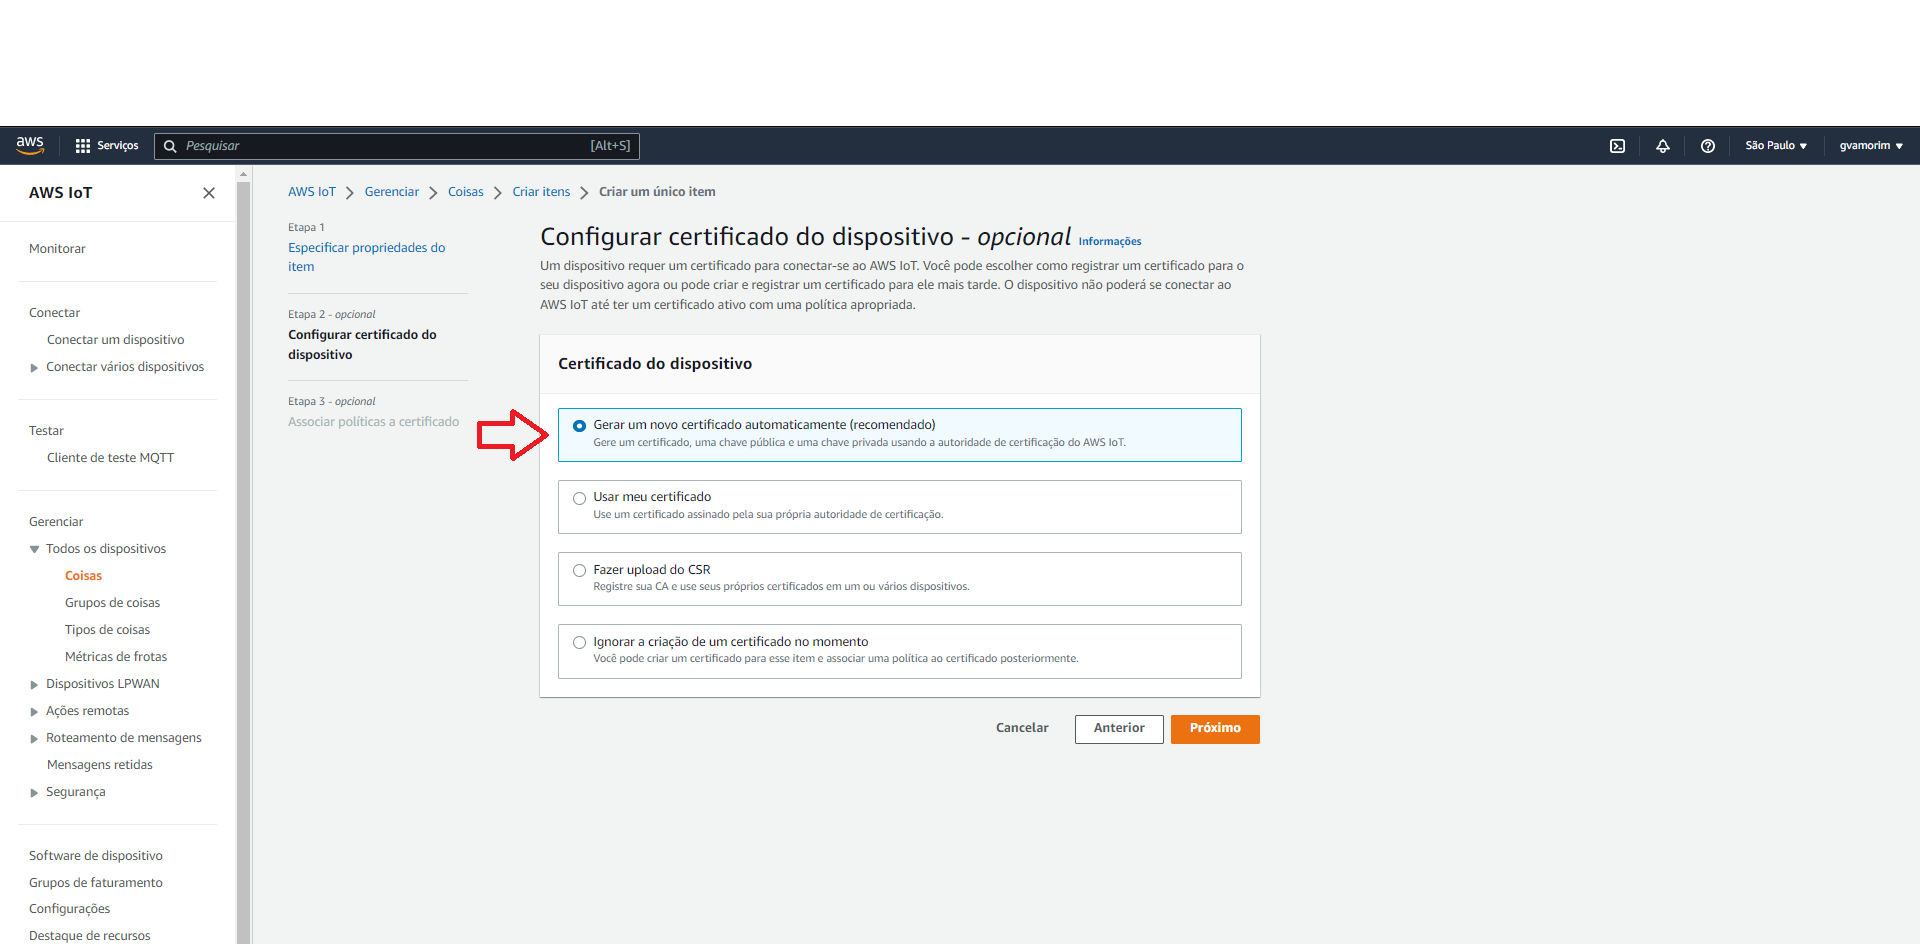
\includegraphics[scale=0.315]{Imagens/criando_uma_coisa_no_aws_iot_4.png}
    \legend{Fonte: Produzido pelo autor (2022).}
\end{figure}

Adicione uma política ao certificado. As políticas do AWS IoT concedem ou negam acesso a recursos do AWS IoT. O processo de criação de uma política para o AWS IoT foi descrito na \autoref{section:criacao_de_uma_politica_para_o_aws_iot}.

\begin{figure}[H]
    \centering
    \caption{Criando uma coisa no AWS IoT (F).}
    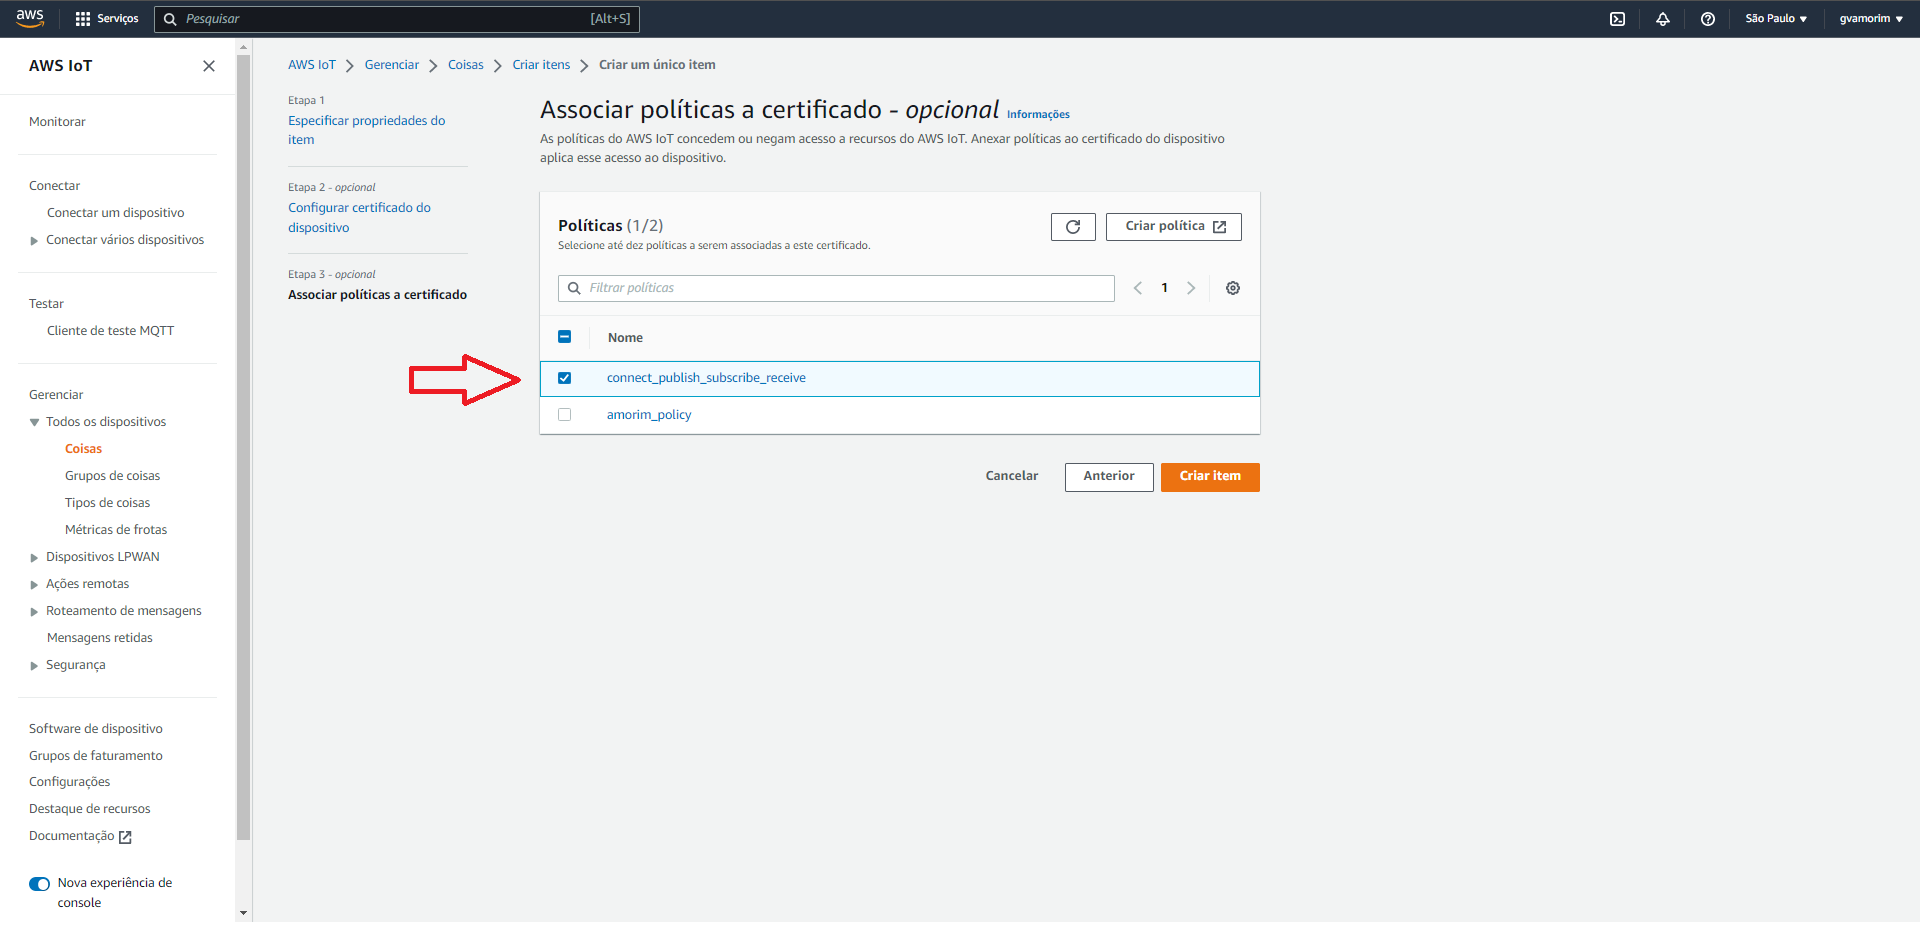
\includegraphics[scale=0.315]{Imagens/criando_uma_coisa_no_aws_iot_5.png}
    \legend{Fonte: Produzido pelo autor (2022).}
\end{figure}

Por fim, a coisa já está pronta no serviço AWS. Faça o \textit{download} dos certificados para que sejam instalados no dispositivo para que este possa se conectar à AWS.

\begin{figure}[H]
    \centering
    \caption{Criando uma coisa no AWS IoT (G).}
    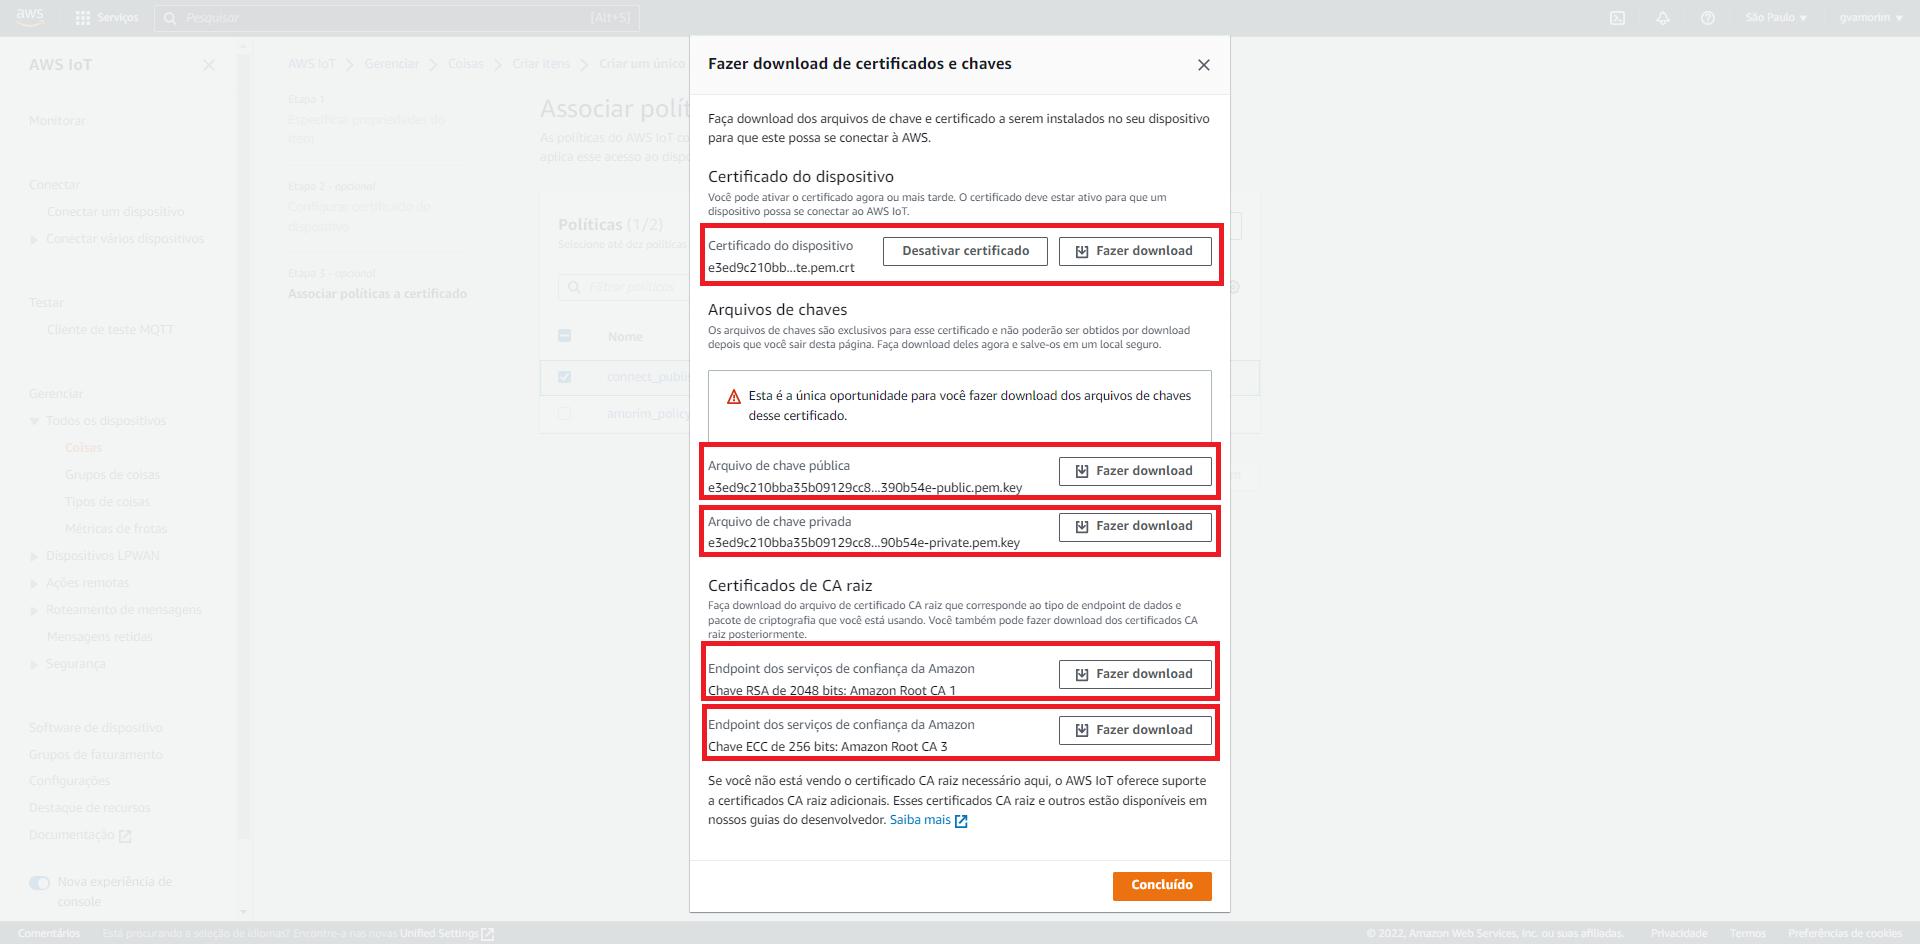
\includegraphics[scale=0.315]{Imagens/criando_uma_coisa_no_aws_iot_6.png}
    \legend{Fonte: Produzido pelo autor (2022).}
    \label{fig:criacao_de_uma_coisa_no_aws_iot_g}
\end{figure}

\section{Configuração do dispositivo B-L475E-IOT01A2 via USB usando o aplicativo Tera Term}\label{section:configuracao_dispositivo_bl475eiot01a2_via_usb}

SEQUÊNCIA DE CAPTURAS DE TELAS DO PROCESSO DE CONFIGURAÇÃO DO DISPOSITIVO B-L475E-IOT01A2 via USB...
